\documentclass[10pt]{article}
 
\usepackage[margin=1in]{geometry} 
\usepackage{amsmath,amsthm,amssymb,amsfonts, graphicx, multicol, array}
\usepackage{mathtools}
\usepackage{booktabs}
\usepackage{stata/stata}
\usepackage{wrapfig}

\graphicspath{ {images/} }

\newcommand\iid{\stackrel{\mathclap{iid}}{\sim}}
\newcommand\asym{\stackrel{\mathclap{a}}{\sim}}
\newcommand\convprob{\xrightarrow{p}}
\newcommand\convdist{\xrightarrow{d}}
\newcommand{\N}{\mathbb{N}}
\newcommand{\Z}{\mathbb{Z}}
\newcommand{\E}{\text{E}}
\newcommand{\V}{\text{Var}}
\newcommand{\Av}{\text{Avar}}
\newcommand{\se}{\text{se}}
\newcommand{\corr}{\text{Corr}}
\newcommand{\cov}{\text{Cov}}
\newcommand{\norm}{\text{Normal}}
\newcommand{\indep}{\perp \!\!\! \perp}
\newcommand{\H}{\text{H}}

 
\newenvironment{problem}[2][Problem]{\begin{trivlist}
\item[\hskip \labelsep {\bfseries #1}\hskip \labelsep {\bfseries #2.}]}{\end{trivlist}}

\begin{document}
 
\title{Homework 3}
\author{ECON 7023: Econometrics II\\
Maghfira Ramadhani\\
February 21, 2022}
\date{Spring 2023}
\maketitle

\section*{Chapter 5}
\subsection*{Problem 5.4}
Use the data in CARD.RAW for this problem
\begin{enumerate}
\item[a.] Estimate a $\log(wage)$ equation by OLS with $educ, exper, exper^2, black, south, smsa, reg661$ through $reg668$, and $smsa66$ as explanatory variables. Compare your results with Table 2, Column (2) in Card (1995).
\\ Answer:
\begin{figure}[h]
    \caption{Result from Card (1995)} \label{Fig3.1}
    \centering
    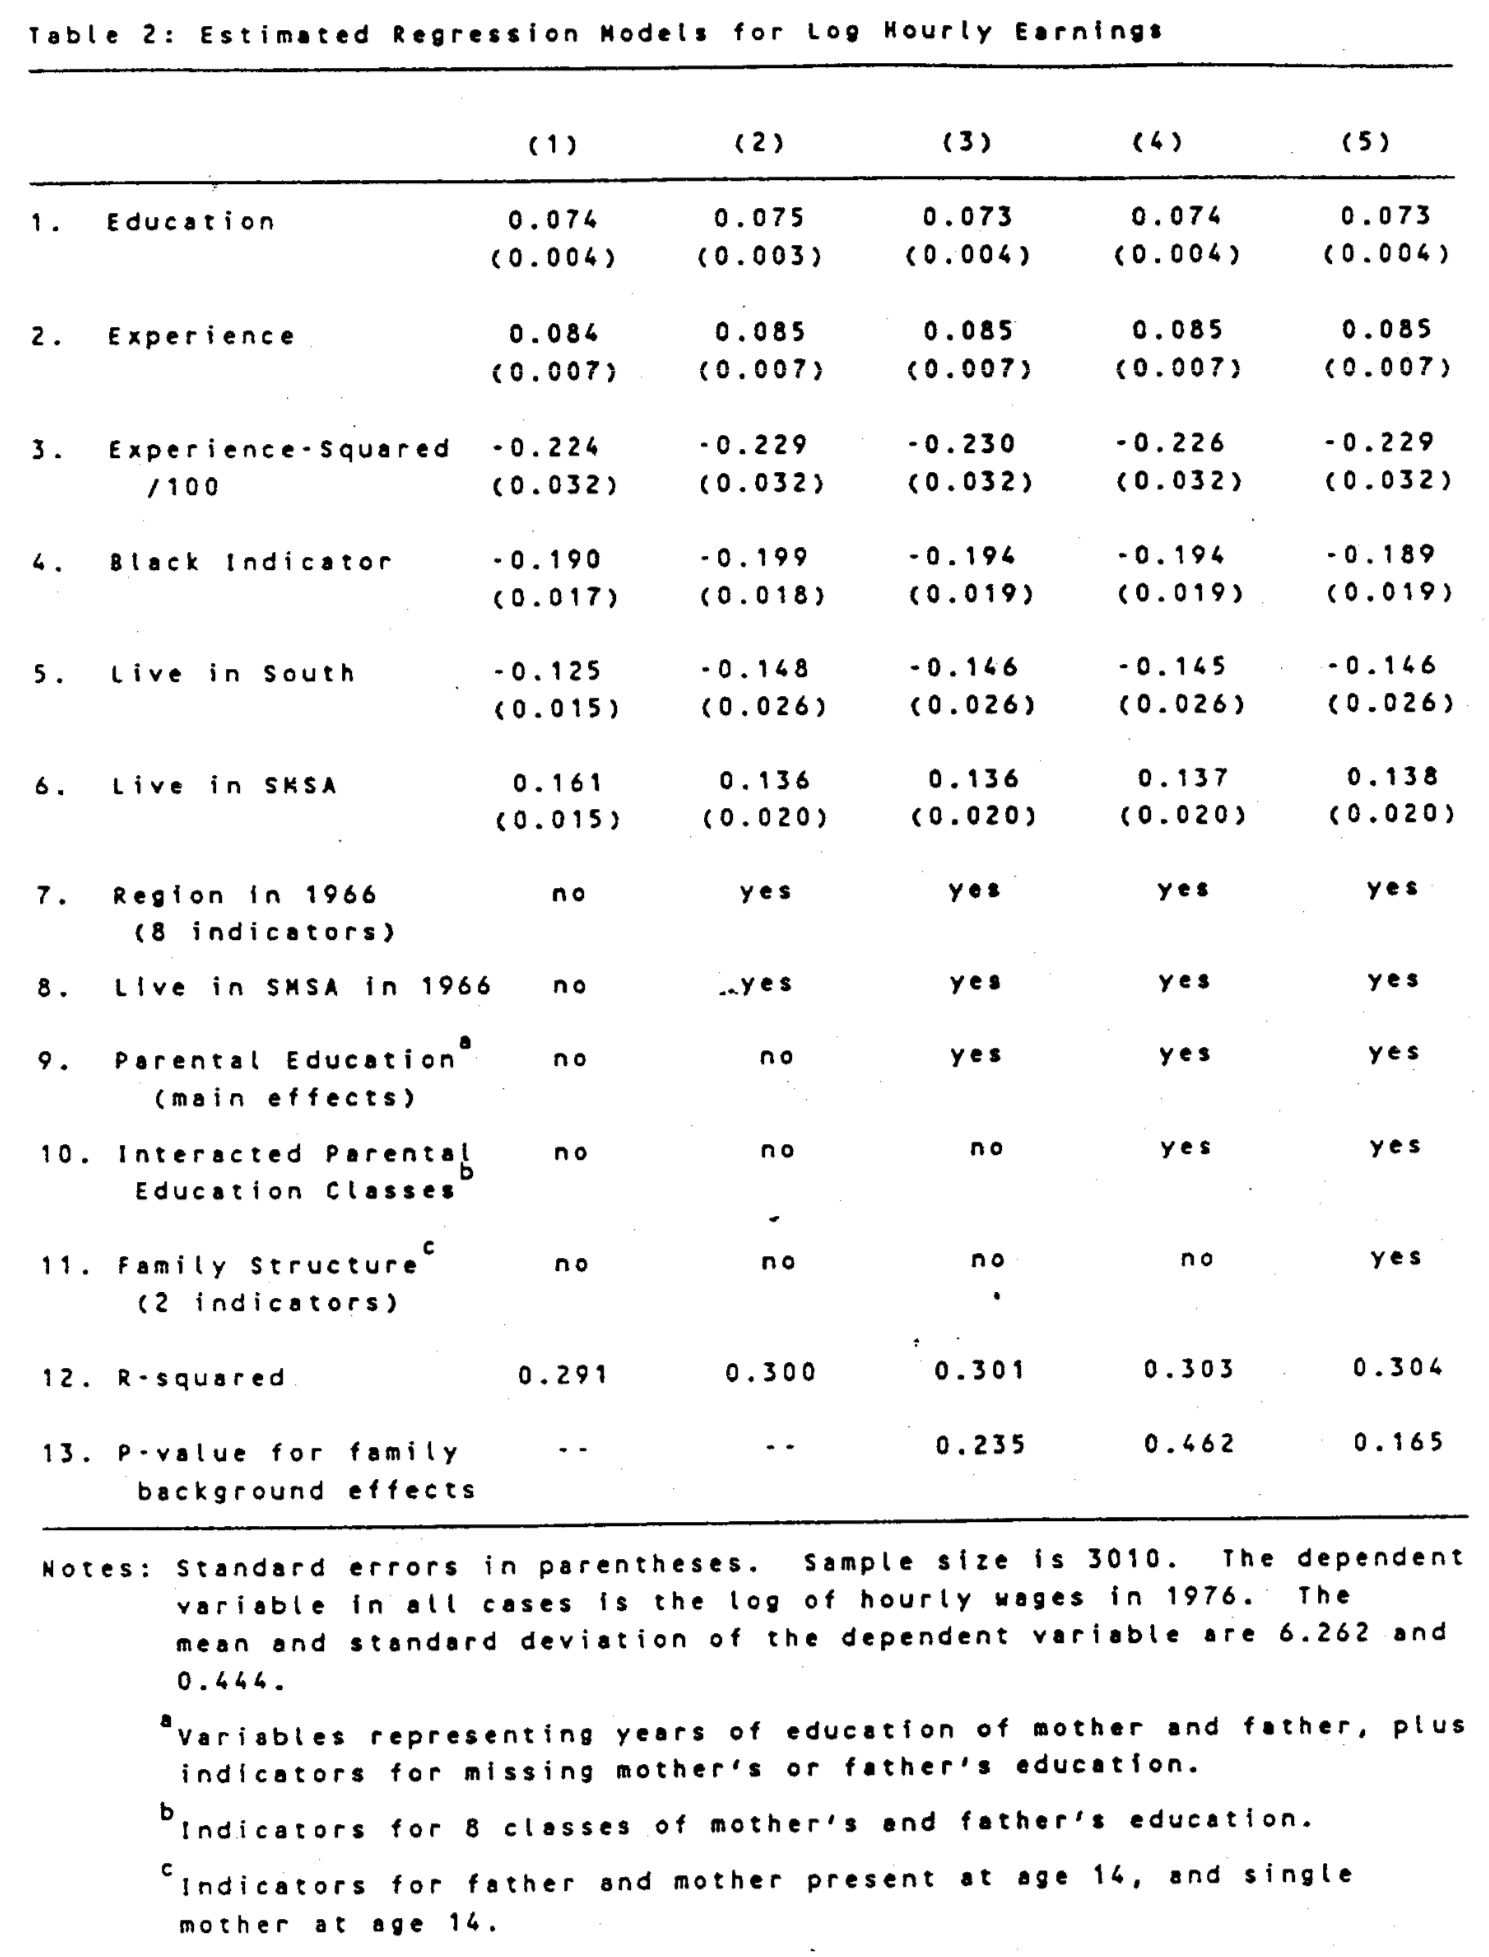
\includegraphics[scale=0.23]{table2.png}
\end{figure}
\\
From Figure \ref{Fig3.1}, we know that the result in Column (2) the return to education is 7.5\% with standard error of 0.03\% and is statistically significant. Comparing to the result that we have in Table 1 from estimating $\log(wage)$ by OLS with $educ, exper, exper^2, black, south, smsa, reg661$ through $reg668$, and $smsa66$ as explanatory variables, we also get 7.5\% return of education with standard error of 0.03\% and is statistically significant. Surprisingly, we get the same coefficient and standard error with those in Card (1995) even though the model specifications are different.
\begin{table}[htbp]\centering
\def\sym#1{\ifmmode^{#1}\else\(^{#1}\)\fi}
\caption{Regression result for Problem 5.4.a.}
\begin{tabular}{l*{1}{c}}
\toprule
                    &\multicolumn{1}{c}{(1)}         \\
\midrule
years of schooling, 1976&       0.075\sym{***}\\
                    &     (0.003)         \\
\addlinespace
age - educ - 6      &       0.085\sym{***}\\
                    &     (0.007)         \\
\addlinespace
exper^2             &      -0.002\sym{***}\\
                    &     (0.000)         \\
\addlinespace
=1 if black         &      -0.199\sym{***}\\
                    &     (0.018)         \\
\addlinespace
=1 if in south, 1976&      -0.148\sym{***}\\
                    &     (0.026)         \\
\addlinespace
=1 in in SMSA, 1976 &       0.136\sym{***}\\
                    &     (0.020)         \\
\addlinespace
regional dummy, 1966&      -0.119\sym{***}\\
                    &     (0.039)         \\
\addlinespace
reg662              &      -0.022         \\
                    &     (0.028)         \\
\addlinespace
reg663              &       0.026         \\
                    &     (0.027)         \\
\addlinespace
reg664              &      -0.063\sym{*}  \\
                    &     (0.036)         \\
\addlinespace
reg665              &       0.009         \\
                    &     (0.036)         \\
\addlinespace
reg666              &       0.022         \\
                    &     (0.040)         \\
\addlinespace
reg667              &      -0.001         \\
                    &     (0.039)         \\
\addlinespace
reg668              &      -0.175\sym{***}\\
                    &     (0.046)         \\
\addlinespace
=1 if in SMSA, 1966 &       0.026         \\
                    &     (0.019)         \\
\addlinespace
Constant            &       4.739\sym{***}\\
                    &     (0.072)         \\
\midrule
Observations        &        3010         \\
\bottomrule
\multicolumn{2}{l}{\footnotesize Standard errors in parentheses}\\
\multicolumn{2}{l}{\footnotesize Data: CARD.DTA}\\
\multicolumn{2}{l}{\footnotesize Wooldridge (2011)}\\
\multicolumn{2}{l}{\footnotesize \sym{*} \(p<0.10\), \sym{**} \(p<0.05\), \sym{***} \(p<0.01\)}\\
\end{tabular}
\end{table}


\item[b.] Estimate a reduced form equation for $educ$ containing all explanatory variables from part a and the dummy variable $nearc4.$ Do $educ$ and $nearc4$ have a practically and statistically significant partial correlation? (See also Table 3, Column (1) in Card (1995).)
\\ Answer:
\begin{figure}[h]
    \caption{Result from Card (1995)} \label{Fig3.2}
    \centering
    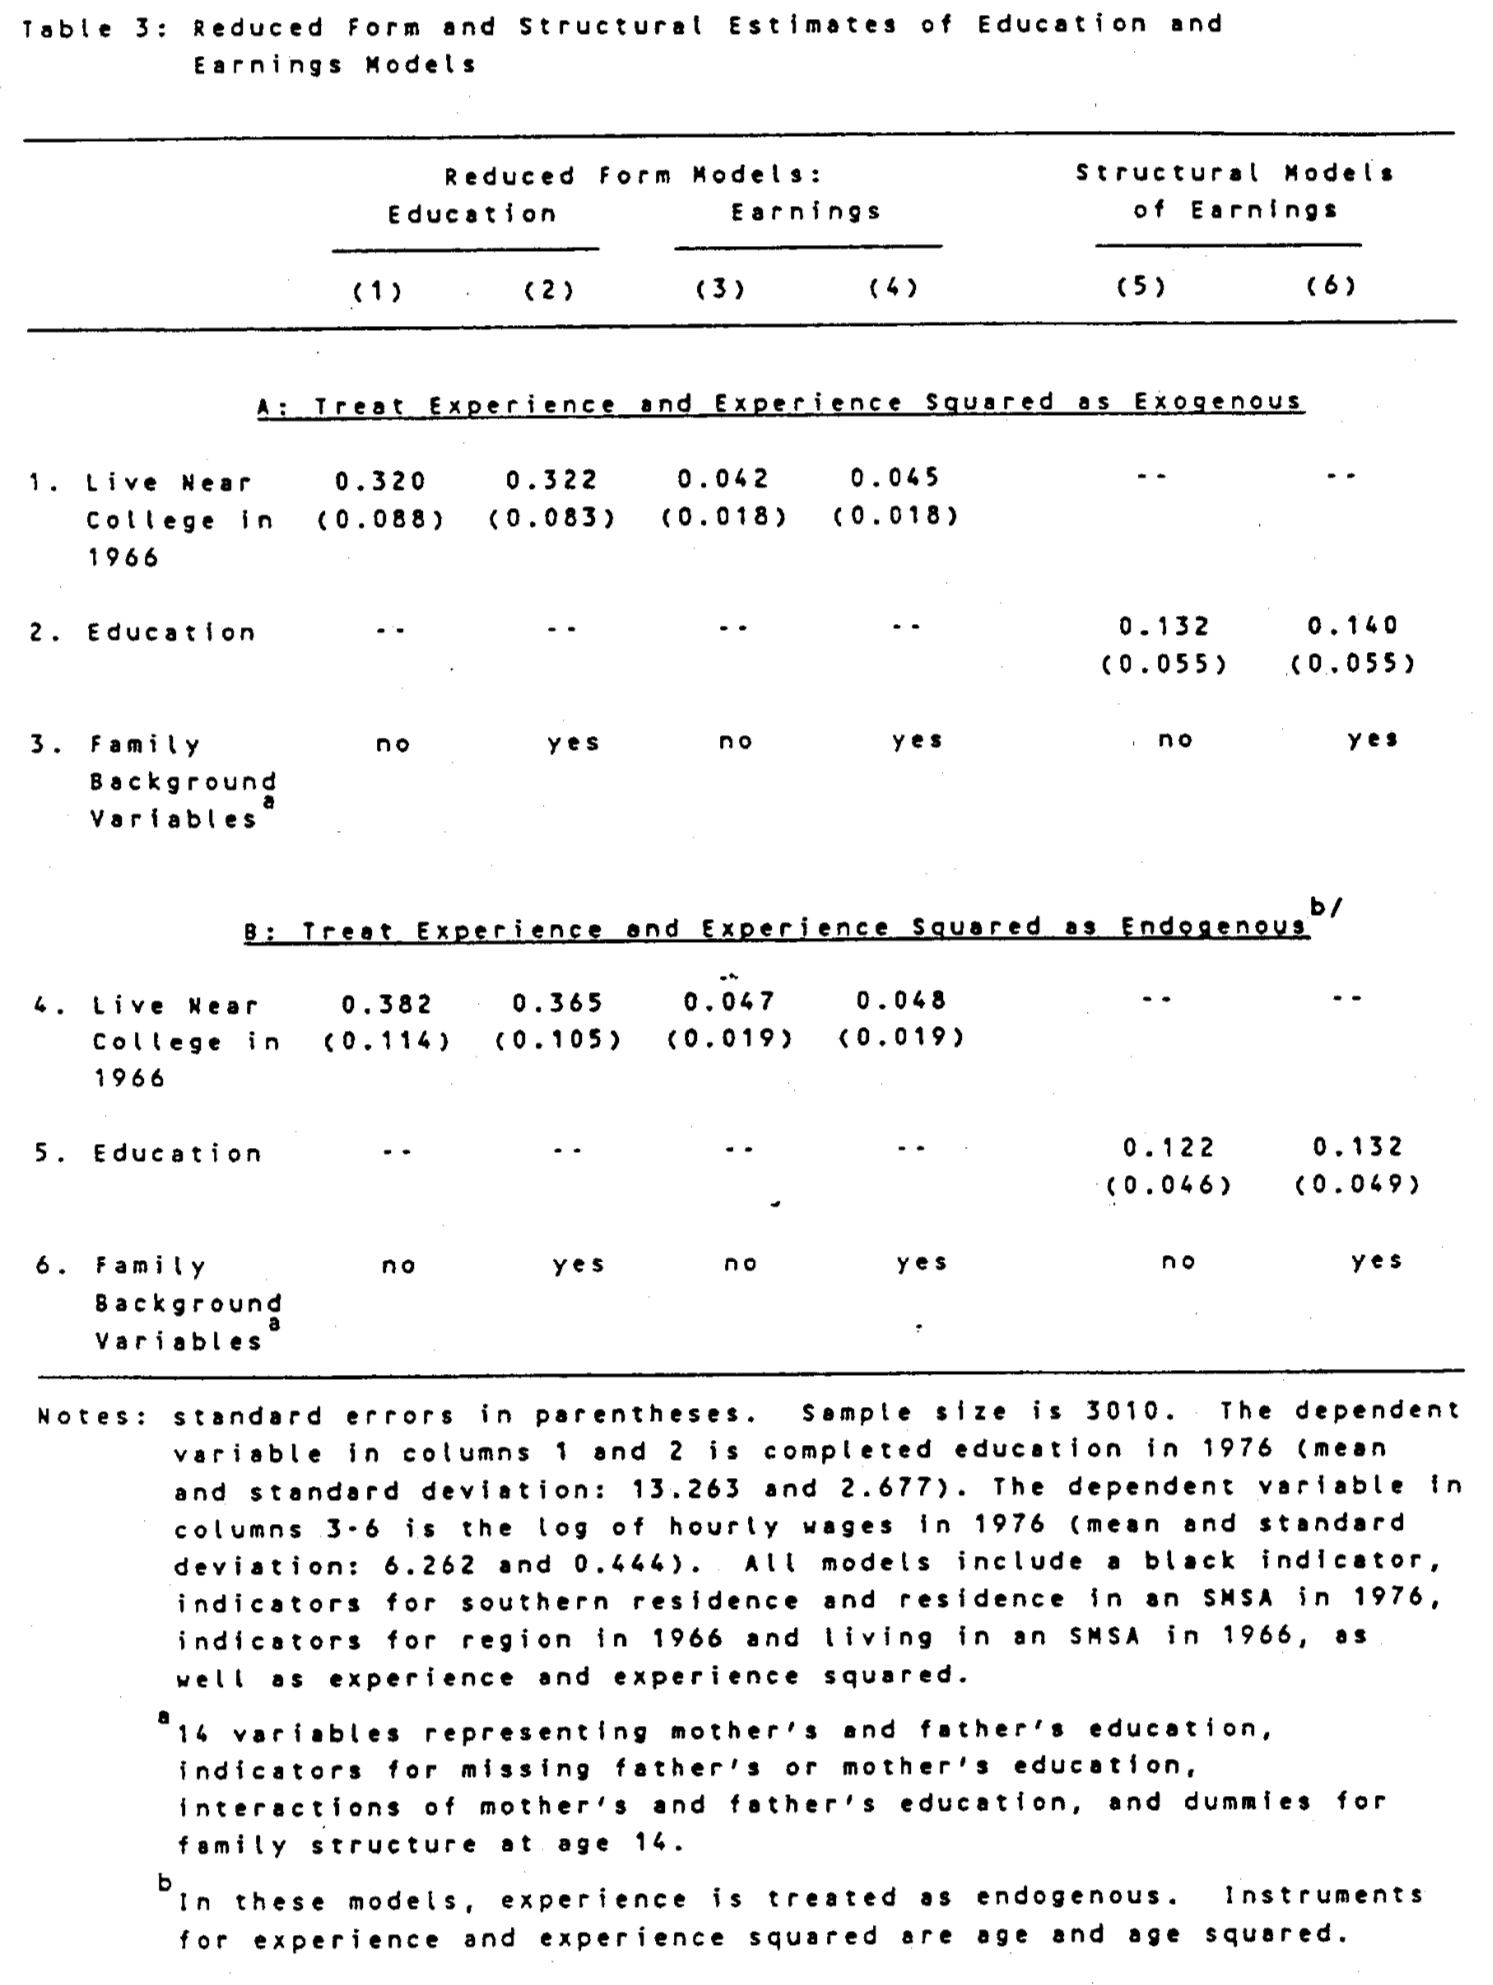
\includegraphics[scale=0.23]{table3.png}
\end{figure}\\
Table 2 Column (1) shows the reduced from estimates for $educ$ containing all explanatory variables from part a and the dummy variable $nearc4.$ Our coefficient of interest is on $nearc4$ which is a dummy variable for someone living near a 4-year college. The estimates show that $educ$ and $nearc4$ are correlated with coefficient of 0.320 with a standard error of 0.0088. The result is statistically very significant. Thus the variable $nearc4$ satisfy the relevance condition for a good IV. Comparing with the result in Card (1995) as shown in Figure \ref{Fig3.2}, the result that we get is the same as in Column (1).
\\
\begin{table}[htbp]\centering
\def\sym#1{\ifmmode^{#1}\else\(^{#1}\)\fi}
\caption{Regression results for (1) Problem 5.4.b. and (2) Problem 5.4.d}
\begin{tabular}{l*{2}{c}}
\toprule
                    &\multicolumn{1}{c}{(1)}         &\multicolumn{1}{c}{(2)}         \\
\midrule
age - educ - 6      &      -0.413\sym{***}&      -0.412\sym{***}\\
                    &     (0.034)         &     (0.034)         \\
\addlinespace
exper^2             &       0.001         &       0.001         \\
                    &     (0.002)         &     (0.002)         \\
\addlinespace
=1 if black         &      -0.936\sym{***}&      -0.945\sym{***}\\
                    &     (0.094)         &     (0.094)         \\
\addlinespace
=1 if in south, 1976&      -0.052         &      -0.042         \\
                    &     (0.135)         &     (0.136)         \\
\addlinespace
=1 in in SMSA, 1976 &       0.402\sym{***}&       0.401\sym{***}\\
                    &     (0.105)         &     (0.105)         \\
\addlinespace
regional dummy, 1966&      -0.210         &      -0.169         \\
                    &     (0.202)         &     (0.204)         \\
\addlinespace
reg662              &      -0.289\sym{**} &      -0.269\sym{*}  \\
                    &     (0.147)         &     (0.148)         \\
\addlinespace
reg663              &      -0.238\sym{*}  &      -0.190         \\
                    &     (0.143)         &     (0.146)         \\
\addlinespace
reg664              &      -0.093         &      -0.038         \\
                    &     (0.186)         &     (0.189)         \\
\addlinespace
reg665              &      -0.483\sym{**} &      -0.437\sym{**} \\
                    &     (0.188)         &     (0.190)         \\
\addlinespace
reg666              &      -0.513\sym{**} &      -0.502\sym{**} \\
                    &     (0.210)         &     (0.210)         \\
\addlinespace
reg667              &      -0.427\sym{**} &      -0.378\sym{*}  \\
                    &     (0.206)         &     (0.208)         \\
\addlinespace
reg668              &       0.314         &       0.382         \\
                    &     (0.242)         &     (0.245)         \\
\addlinespace
=1 if in SMSA, 1966 &       0.025         &       0.000         \\
                    &     (0.106)         &     (0.107)         \\
\addlinespace
=1 if near 4 yr college, 1966&       0.320\sym{***}&       0.321\sym{***}\\
                    &     (0.088)         &     (0.088)         \\
\addlinespace
=1 if near 2 yr college, 1966&                     &       0.123         \\
                    &                     &     (0.077)         \\
\addlinespace
Constant            &      16.849\sym{***}&      16.773\sym{***}\\
                    &     (0.211)         &     (0.216)         \\
\midrule
Observations        &        3010         &        3010         \\
\bottomrule
\multicolumn{3}{l}{\footnotesize Standard errors in parentheses}\\
\multicolumn{3}{l}{\footnotesize Data: CARD.DTA}\\
\multicolumn{3}{l}{\footnotesize Wooldridge (2011)}\\
\multicolumn{3}{l}{\footnotesize \sym{*} \(p<0.10\), \sym{**} \(p<0.05\), \sym{***} \(p<0.01\)}\\
\end{tabular}
\end{table}


\item[c.] Estimate the $\log(wage)$ equation by IV, using $nearc4$ as an instrument for $educ.$ Compare the 95 percent confidence interval for the return to education with that obtained from part a. (See also Table 3, Column (5) in Card (1995).)
\\ Answer:\\
Table 3 Column (1) shows the $\log(wage)$ equation by IV, using $nearc4$ as an instrument for $educ.$ The estimated return to education that we get is 13.2\% with standard error of 5.5\%. The 95 percent confidence in the 2SLS estimation is 2.37\% to 23.93\% while in the OLS estimation it is 6.78\% to 8.15\%. In this case, in the OLS since there is indication of endogeneity problem, the estimator may be inconsistent even though the confidence interval is smaller but we still can not believe it directly. 
\\ \\
OLS Regression
\begin{stlog}. reg lwage educ exper expersq black south smsa reg661-reg668 smsa66
{\smallskip}
      Source {\VBAR}       SS           df       MS      Number of obs   =     3,010
\HLI{13}{\PLUS}\HLI{34}   F(15, 2994)     =     85.48
       Model {\VBAR}  177.695591        15  11.8463727   Prob > F        =    0.0000
    Residual {\VBAR}  414.946054     2,994  .138592536   R-squared       =    0.2998
\HLI{13}{\PLUS}\HLI{34}   Adj R-squared   =    0.2963
       Total {\VBAR}  592.641645     3,009  .196956346   Root MSE        =    .37228
{\smallskip}
\HLI{13}{\TOPT}\HLI{64}
       lwage {\VBAR} Coefficient  Std. err.      t    P>|t|     [95\% conf. interval]
\HLI{13}{\PLUS}\HLI{64}
        educ {\VBAR}   .0746933   .0034983    21.35   0.000     .0678339    .0815527
       exper {\VBAR}    .084832   .0066242    12.81   0.000     .0718435    .0978205
     expersq {\VBAR}   -.002287   .0003166    -7.22   0.000    -.0029079   -.0016662
       black {\VBAR}  -.1990123   .0182483   -10.91   0.000    -.2347927   -.1632318
       south {\VBAR}   -.147955   .0259799    -5.69   0.000    -.1988952   -.0970148
        smsa {\VBAR}   .1363845   .0201005     6.79   0.000     .0969724    .1757967
      reg661 {\VBAR}  -.1185698   .0388301    -3.05   0.002     -.194706   -.0424335
      reg662 {\VBAR}  -.0222026   .0282575    -0.79   0.432    -.0776088    .0332036
      reg663 {\VBAR}   .0259703   .0273644     0.95   0.343    -.0276846    .0796251
      reg664 {\VBAR}  -.0634942   .0356803    -1.78   0.075    -.1334546    .0064662
      reg665 {\VBAR}   .0094551   .0361174     0.26   0.794    -.0613623    .0802725
      reg666 {\VBAR}   .0219476   .0400984     0.55   0.584    -.0566755    .1005708
      reg667 {\VBAR}  -.0005887   .0393793    -0.01   0.988     -.077802    .0766245
      reg668 {\VBAR}  -.1750058   .0463394    -3.78   0.000     -.265866   -.0841456
      smsa66 {\VBAR}   .0262417   .0194477     1.35   0.177    -.0118905    .0643739
       _cons {\VBAR}   4.739377   .0715282    66.26   0.000     4.599127    4.879626
\HLI{13}{\BOTT}\HLI{64}
{\smallskip}
\end{stlog}

2SLS Regression using $nearc4$ as instrument for $educ$
\begin{stlog}. ivreg lwage exper expersq black south smsa reg661-reg668 smsa66 (educ = nearc4)
{\smallskip}
Instrumental variables 2SLS regression
{\smallskip}
      Source {\VBAR}       SS           df       MS      Number of obs   =     3,010
\HLI{13}{\PLUS}\HLI{34}   F(15, 2994)     =     51.01
       Model {\VBAR}  141.146813        15  9.40978752   Prob > F        =    0.0000
    Residual {\VBAR}  451.494832     2,994  .150799877   R-squared       =    0.2382
\HLI{13}{\PLUS}\HLI{34}   Adj R-squared   =    0.2343
       Total {\VBAR}  592.641645     3,009  .196956346   Root MSE        =    .38833
{\smallskip}
\HLI{13}{\TOPT}\HLI{64}
       lwage {\VBAR} Coefficient  Std. err.      t    P>|t|     [95\% conf. interval]
\HLI{13}{\PLUS}\HLI{64}
        educ {\VBAR}   .1315038   .0549637     2.39   0.017     .0237335    .2392742
       exper {\VBAR}   .1082711   .0236586     4.58   0.000     .0618824    .1546598
     expersq {\VBAR}  -.0023349   .0003335    -7.00   0.000    -.0029888    -.001681
       black {\VBAR}  -.1467757   .0538999    -2.72   0.007    -.2524603   -.0410912
       south {\VBAR}  -.1446715   .0272846    -5.30   0.000      -.19817    -.091173
        smsa {\VBAR}   .1118083    .031662     3.53   0.000     .0497269    .1738898
      reg661 {\VBAR}  -.1078142   .0418137    -2.58   0.010    -.1898007   -.0258278
      reg662 {\VBAR}  -.0070465   .0329073    -0.21   0.830    -.0715696    .0574767
      reg663 {\VBAR}   .0404445   .0317806     1.27   0.203    -.0218694    .1027585
      reg664 {\VBAR}  -.0579172   .0376059    -1.54   0.124    -.1316532    .0158189
      reg665 {\VBAR}   .0384577   .0469387     0.82   0.413    -.0535777     .130493
      reg666 {\VBAR}   .0550887   .0526597     1.05   0.296    -.0481642    .1583416
      reg667 {\VBAR}    .026758   .0488287     0.55   0.584    -.0689832    .1224992
      reg668 {\VBAR}  -.1908912   .0507113    -3.76   0.000    -.2903238   -.0914586
      smsa66 {\VBAR}   .0185311   .0216086     0.86   0.391    -.0238381    .0609003
       _cons {\VBAR}   3.773965    .934947     4.04   0.000     1.940762    5.607169
\HLI{13}{\BOTT}\HLI{64}
Instrumented: educ
 Instruments: exper expersq black south smsa reg661 reg662 reg663 reg664
              reg665 reg666 reg667 reg668 smsa66 nearc4
{\smallskip}
\end{stlog}

\begin{table}[htbp]\centering
\def\sym#1{\ifmmode^{#1}\else\(^{#1}\)\fi}
\caption{Regression result for Problem 5.4.c.}
\begin{tabular}{l*{1}{c}}
\toprule
                    &\multicolumn{1}{c}{(1)}         \\
\midrule
years of schooling, 1976&       0.132\sym{**} \\
                    &     (0.055)         \\
\addlinespace
age - educ - 6      &       0.108\sym{***}\\
                    &     (0.024)         \\
\addlinespace
exper^2             &      -0.002\sym{***}\\
                    &     (0.000)         \\
\addlinespace
=1 if black         &      -0.147\sym{***}\\
                    &     (0.054)         \\
\addlinespace
=1 if in south, 1976&      -0.145\sym{***}\\
                    &     (0.027)         \\
\addlinespace
=1 in in SMSA, 1976 &       0.112\sym{***}\\
                    &     (0.032)         \\
\addlinespace
regional dummy, 1966&      -0.108\sym{***}\\
                    &     (0.042)         \\
\addlinespace
reg662              &      -0.007         \\
                    &     (0.033)         \\
\addlinespace
reg663              &       0.040         \\
                    &     (0.032)         \\
\addlinespace
reg664              &      -0.058         \\
                    &     (0.038)         \\
\addlinespace
reg665              &       0.038         \\
                    &     (0.047)         \\
\addlinespace
reg666              &       0.055         \\
                    &     (0.053)         \\
\addlinespace
reg667              &       0.027         \\
                    &     (0.049)         \\
\addlinespace
reg668              &      -0.191\sym{***}\\
                    &     (0.051)         \\
\addlinespace
=1 if in SMSA, 1966 &       0.019         \\
                    &     (0.022)         \\
\addlinespace
Constant            &       3.774\sym{***}\\
                    &     (0.935)         \\
\midrule
Observations        &        3010         \\
\bottomrule
\multicolumn{2}{l}{\footnotesize Standard errors in parentheses}\\
\multicolumn{2}{l}{\footnotesize Data: CARD.DTA}\\
\multicolumn{2}{l}{\footnotesize Wooldridge (2011)}\\
\multicolumn{2}{l}{\footnotesize \sym{*} \(p<0.10\), \sym{**} \(p<0.05\), \sym{***} \(p<0.01\)}\\
\end{tabular}
\end{table}



\item[d.] Now use $nearc2$ along with $nearc4$ as instruments for $educ$. First estimate the reduced form for $educ$, and comment on whether $nearc4$ is more strongly related to $educ$. How do the 2SLS estimates compare with the earlier estimates?
\\ Answer:\\
Table 2 Column (2) shows the reduced form estimates when adding $nearc2$ and $nearc4$ together. The coefficient for $nearc2$ is 0.123 with standard error of 0.077 which is not statistically significant. Compared to previous result, the coefficient for $nearc4$ is now increased to 0.321 with relatively similar standard error. Table 3 Column (2) shows the 2SLS estimates with $nearc2$ and $nearc4$ as instruments. The return to education increase to about 15.7\% with increased significance level compared to previous result when using only $nearc4$.



\item[e.] For as subset of the men in the sample, IQ score is available. Regress $iq$ on $nearc4.$ Is IQ score uncorrelated with $nearc4$?
\\ Answer:\\
Table 4 Column (1) show the regression result, it shows that IQ score is correlated with $nearc4.$ 
\begin{table}[htbp]\centering
\def\sym#1{\ifmmode^{#1}\else\(^{#1}\)\fi}
\caption{Regression results for (1) Problem 5.4.e. and (2) Problem 5.4.f.}
\begin{tabular}{l*{2}{c}}
\toprule
                    &\multicolumn{1}{c}{(1)}         &\multicolumn{1}{c}{(2)}         \\
\midrule
=1 if near 4 yr college, 1966&       2.596\sym{***}&       0.868         \\
                    &     (0.745)         &     (0.822)         \\
\addlinespace
=1 if in SMSA, 1966 &                     &       1.355\sym{*}  \\
                    &                     &     (0.803)         \\
\addlinespace
regional dummy, 1966&                     &       4.768\sym{***}\\
                    &                     &     (1.547)         \\
\addlinespace
reg662              &                     &       5.808\sym{***}\\
                    &                     &     (0.902)         \\
\addlinespace
reg669              &                     &       1.845         \\
                    &                     &     (1.152)         \\
\addlinespace
Constant            &     100.611\sym{***}&      99.385\sym{***}\\
                    &     (0.627)         &     (0.702)         \\
\midrule
Observations        &        2061         &        2061         \\
\bottomrule
\multicolumn{3}{l}{\footnotesize Standard errors in parentheses}\\
\multicolumn{3}{l}{\footnotesize Data: CARD.DTA}\\
\multicolumn{3}{l}{\footnotesize Wooldridge (2011)}\\
\multicolumn{3}{l}{\footnotesize \sym{*} \(p<0.10\), \sym{**} \(p<0.05\), \sym{***} \(p<0.01\)}\\
\end{tabular}
\end{table}


\item[f.] Now regress $iq$ on $nearc4$ along with $smsa66, reg661, reg662,$ and $reg669.$ Are $iq$ and $nearc4$ partially correlated? What do you conclude about the importance of controlling for the 1966 location and regional dummies in the $\log(wage)$ equation when using $nearc4$ as an IV for $educ$?
\\ Answer:\\
Table 4 Column (2) show the regression result, now after controlling for $smsa66, reg661, reg662,$ and $reg669$ the coefficient on $nearc4$ become insignificant, in other word the effect or correlation still exists and the same, but statistically dissapears. Thus, when using $nearc4$ as IV for educ, it is important to add control variables also in the $\log(wage)$ equation.
\end{enumerate}


\subsection*{Problem 5.7}
Consider model (5.45) where $v$ has zero mean and is uncorrelated with $x_1,\ldots,x_K$ and $q$. The unobservable $q$ is thought to be correlated with at least some of the $x_j$. Assume without loss of generality that $\E(q)=0.$\\
You have a single indicator of $q$, written as $q_1=\delta_1q+a_1,\delta_1\neq 0,$ where $a_1$ has zero mean and is uncorrelated with each of $x_j,q$ and $v$. In addition, $z_1,z_2,\ldots,z_M$ is a set of variables that are (1) redundant in the structural equation (5.45) and (2) uncorrelated with $a_1.$
\begin{enumerate}
\item[a.] Suggest an IV method for consistently estimating the $\beta_j.$ Be sure to discuss what is needed for identification.
\\ Answer:\\
Recall equation (5.45)
\[y=\beta_0+\beta_1x_1+\cdots+\beta_Kx_K+\gamma q+v.\]
It is given that $q_1=\delta_1q+a_1 \Leftrightarrow q=\frac{1}{\delta_1}q_1-\frac{1}{\delta_1}a_1$. Substitute it to (5.45) we will have
\begin{align}
    y&=\beta_0+\beta_1x_1+\cdots+\beta_Kx_K+\gamma \left(\frac{1}{\delta_1}q_1-\frac{1}{\delta_1}a_1\right)+v \notag \\
    y&=\beta_0+\beta_1x_1+\cdots+\beta_Kx_K+\frac{\gamma}{\delta_1}q_1+v-\frac{\gamma}{\delta_1}a_1 \label{h3.1}
\end{align}
We also have $z_1,z_2,\ldots,z_M$ is a set of variables that are redundant in the structural equation (5.45) and uncorrelated with $a_1.$ Thus, we have $z_1,z_2,\ldots,z_M$ are uncorrelated with the error, $v$. Also, $a_1$ is uncorrelated with each of $x_j,q$ and $v$. Thus, we have $x_j$ uncorrelated with $v-\frac{\gamma}{\delta_1}a_1.$ These conditions satisfy the exlclusion conditions for IV. Therefore we can now estimate equation \eqref{h3.1} to get consistent estimation for $\beta_j$ and $\frac{\gamma}{\delta_1}$ by 2SLS estimation using instruments $x_1,\ldots,x_K,z_1,\ldots,z_M.$ Another identification that we need to show is that at least one of the instruments in $z_1,\ldots,z_M$ appears in $q_1$ to satisfy the rank condition.

\item[b.] If equation (5.45) is a $\log(wage)$ equation, $q$ is ability, $q_1$ is IQ or some other test score, and $z_1,\ldots,z_M$ are family of variables, such as parents' education and number of siblings, describe the economic assumption needed for consistency of the IV procedure in part a.
\\ Answer:\\
Suppose $y$ is $\log(wage)$, $z_1,\ldots,z_M$ are family of variables, such as parents' education and number of siblings. The first condition is for family background to be exogenous in equation (5.45), or that the family backgrounds variables are redundant in (5.45) after we control for ability using the indicator $q_1$. The second condition, the rank condition, we need the family backgrounds variable to be correlated with the indicator $q_1$ or $IQ$. It is common to say that family background will be partially correlated with ability.

\item[c.] Carry out this procedure using the data in NLS80.RAW. Include among the explanatory variables $exper, tenure,educ,married,south,urban,$ and $black$. First use $IQ$ as $q_1$ and then $KWW$. Include in the $z_h$ the variables $meduc,feduc,$ and $sibs.$ Discuss the results.
\\ Answer:\\
2SLS Regression using $meduc, feduc, sibs$ as instrument for $iq$
\begin{stlog}. ivreg lwage exper tenure educ married south urban black (iq = meduc feduc sibs)
{\smallskip}
Instrumental variables 2SLS regression
{\smallskip}
      Source {\VBAR}       SS           df       MS      Number of obs   =       722
\HLI{13}{\PLUS}\HLI{34}   F(8, 713)       =     25.81
       Model {\VBAR}  19.6029198         8  2.45036497   Prob > F        =    0.0000
    Residual {\VBAR}  107.208996       713  .150363248   R-squared       =    0.1546
\HLI{13}{\PLUS}\HLI{34}   Adj R-squared   =    0.1451
       Total {\VBAR}  126.811916       721  .175883378   Root MSE        =    .38777
{\smallskip}
\HLI{13}{\TOPT}\HLI{64}
       lwage {\VBAR} Coefficient  Std. err.      t    P>|t|     [95\% conf. interval]
\HLI{13}{\PLUS}\HLI{64}
          iq {\VBAR}   .0154368   .0077077     2.00   0.046     .0003044    .0305692
       exper {\VBAR}   .0162185   .0040076     4.05   0.000     .0083503    .0240867
      tenure {\VBAR}   .0076754   .0030956     2.48   0.013     .0015979    .0137529
        educ {\VBAR}   .0161809   .0261982     0.62   0.537     -.035254    .0676158
     married {\VBAR}   .1901012   .0467592     4.07   0.000     .0982991    .2819033
       south {\VBAR}   -.047992   .0367425    -1.31   0.192    -.1201284    .0241444
       urban {\VBAR}   .1869376   .0327986     5.70   0.000     .1225442    .2513311
       black {\VBAR}   .0400269   .1138678     0.35   0.725    -.1835294    .2635832
       _cons {\VBAR}   4.471616    .468913     9.54   0.000        3.551    5.392231
\HLI{13}{\BOTT}\HLI{64}
Instrumented: iq
 Instruments: exper tenure educ married south urban black meduc feduc sibs
{\smallskip}
\end{stlog}
2SLS Regression using $meduc, feduc, sibs$ as instrument for $kww$
\begin{stlog}. ivreg lwage tenure educ married south urban black (kww = meduc feduc sibs)
{\smallskip}
Instrumental variables 2SLS regression
{\smallskip}
      Source {\VBAR}       SS           df       MS      Number of obs   =       722
\HLI{13}{\PLUS}\HLI{34}   F(7, 714)       =     27.70
       Model {\VBAR}  22.0383042         7  3.14832917   Prob > F        =    0.0000
    Residual {\VBAR}  104.773612       714  .146741753   R-squared       =    0.1738
\HLI{13}{\PLUS}\HLI{34}   Adj R-squared   =    0.1657
       Total {\VBAR}  126.811916       721  .175883378   Root MSE        =    .38307
{\smallskip}
\HLI{13}{\TOPT}\HLI{64}
       lwage {\VBAR} Coefficient  Std. err.      t    P>|t|     [95\% conf. interval]
\HLI{13}{\PLUS}\HLI{64}
         kww {\VBAR}    .022462    .014171     1.59   0.113    -.0053598    .0502838
      tenure {\VBAR}   .0072688   .0043559     1.67   0.096     -.001283    .0158207
        educ {\VBAR}   .0237309   .0198777     1.19   0.233    -.0152949    .0627567
     married {\VBAR}   .1722297   .0541382     3.18   0.002     .0659407    .2785187
       south {\VBAR}  -.0934557   .0316378    -2.95   0.003      -.15557   -.0313414
       urban {\VBAR}   .1533135   .0403009     3.80   0.000      .074191     .232436
       black {\VBAR}  -.0561141   .0864972    -0.65   0.517    -.2259333    .1137051
       _cons {\VBAR}   5.389126   .2175243    24.77   0.000     4.962062    5.816189
\HLI{13}{\BOTT}\HLI{64}
Instrumented: kww
 Instruments: tenure educ married south urban black meduc feduc sibs
{\smallskip}
\end{stlog}
.   
\begin{table}[htbp]\centering
\def\sym#1{\ifmmode^{#1}\else\(^{#1}\)\fi}
\caption{Regression results for Problem 5.7.c.}
\begin{tabular}{l*{2}{c}}
\toprule
                    &\multicolumn{1}{c}{(1)}         &\multicolumn{1}{c}{(2)}         \\
\midrule
IQ score            &       0.015\sym{**} &                     \\
                    &     (0.008)         &                     \\
\addlinespace
years of work experience&       0.016\sym{***}&       0.007         \\
                    &     (0.004)         &     (0.007)         \\
\addlinespace
years with current employer&       0.008\sym{**} &       0.005         \\
                    &     (0.003)         &     (0.004)         \\
\addlinespace
years of education  &       0.016         &       0.026         \\
                    &     (0.026)         &     (0.026)         \\
\addlinespace
=1 if married       &       0.190\sym{***}&       0.161\sym{***}\\
                    &     (0.047)         &     (0.053)         \\
\addlinespace
=1 if live in south &      -0.048         &      -0.092\sym{***}\\
                    &     (0.037)         &     (0.032)         \\
\addlinespace
=1 if live in SMSA  &       0.187\sym{***}&       0.148\sym{***}\\
                    &     (0.033)         &     (0.041)         \\
\addlinespace
=1 if black         &       0.040         &      -0.042         \\
                    &     (0.114)         &     (0.089)         \\
\addlinespace
knowledge of world work score&                     &       0.025\sym{*}  \\
                    &                     &     (0.015)         \\
\addlinespace
Constant            &       4.472\sym{***}&       5.218\sym{***}\\
                    &     (0.469)         &     (0.163)         \\
\midrule
Observations        &         722         &         722         \\
\bottomrule
\multicolumn{3}{l}{\footnotesize Standard errors in parentheses}\\
\multicolumn{3}{l}{\footnotesize Data: NLS80.DTA}\\
\multicolumn{3}{l}{\footnotesize Wooldridge (2011)}\\
\multicolumn{3}{l}{\footnotesize \sym{*} \(p<0.10\), \sym{**} \(p<0.05\), \sym{***} \(p<0.01\)}\\
\end{tabular}
\end{table}

\end{enumerate}

\subsection*{Problem 5.11}
A model with a single endogenous explanatory variable can be written as
\[y_1=\textbf{z}_1\pmb{\delta}_1+\alpha_1y_2+u_1, \ \ \ \E(\textbf{z}'u_1)=0,\]
where $\textbf{z}=(\textbf{z}_1,\textbf{z}_2)$. Consider the following two-step method, intended to mimic 2SLS:
\begin{enumerate}
    \item[a.] Regress $y_2$ on $\textbf{z}_2$, and obtain the fitted values, $\Tilde{y}_2$. (That is, $\textbf{z}_1$ is omitted from the first-stage regression.)
    \item[b.] Regress $y_1$ on $\textbf{z}_1, \Tilde{y}_2$ to obtain $\Tilde{\pmb{\delta}}_1$ and $\Tilde{\alpha}_1$. 
\end{enumerate}
Show that $\Tilde{\pmb{\delta}}_1$ and $\Tilde{\alpha}_1$ are generally inconsistent. When would $\Tilde{\pmb{\delta}}_1$ and $\Tilde{\alpha}_1$ be consistent? (Hint: Let $y_2^0$ be the population linear projection of $y_2$ on $\textbf{z}_2$, and let $a_2$ be the projection error: $y_2^0=\textbf{z}_2\pmb{\lambda}_2+a_2, \E(\textbf{z}_2'a_2)=\textbf{0}$. For simplicity, pretend that $\pmb{\lambda}_2$ is known rather than estimated; that is, assume that $\Tilde{y}_2$ is actually $y_2^0.$ Then, write:
\[y_1=\textbf{z}_1\pmb{\delta}_1+\alpha_1y_2^0+\alpha_1a_2+u_1\]
and check whether the composite error $\alpha_1a_2+u_1$ is uncorrelated with the explanatory variables.)
\\ Answer:\\
Following the hint, let $y_2^0$ be the population linear projection of $y_2$ on $\textbf{z}_2$, and let $a_2$ be the projection error: $y_2^0=\textbf{z}_2\pmb{\lambda}_2+a_2, \E(\textbf{z}_2'a_2)=\textbf{0}$. Assume that $\pmb{\lambda}_2$ is known. Write $y_2=y_2^0+a_2$ and substitute it into the original equation, we have
\begin{align*}
    &y_1=\textbf{z}_1\pmb{\delta}_1+\alpha_1y_2+u_1 \\
    &\Leftrightarrow y_1=\textbf{z}_1\pmb{\delta}_1+\alpha_1(y_2^0+a_2)+u_1 \\
    &\Leftrightarrow y_1=\textbf{z}_1\pmb{\delta}_1+\alpha_1y_2^0+\underbrace{\alpha_1 a_2+u_1}_{\displaystyle \text{composite error}}.
\end{align*}
The conditions for consistent estimation is that $\alpha_1 a_2+u_1$ be orthogonal to $\textbf{z}_1$ and $y_2^0$. It is given that $E(\textbf{z}'u_1)=0$ which also means $E(\textbf{z}'_1u_1)=0,E(\textbf{z}'_2u_1)=0$. From the linear projection by construction we have $E(\textbf{z}'_2a_2)=0$. However, since $\textbf{z}_1$ is omitted in step a, we will have $E(\textbf{z}'_2a_2)\neq0$. Thus our OLS regression in step b will produce inconsistent estimation. This problem happens because we did not include all exogenous variable in the first stage regression.

\subsection*{Problem 5.13}
Consider the simple regression model
\[y=\beta_1+\beta_1x+u\]
and let $z$ be a \textit{binary} instrumental variable for $x.$ 
\begin{enumerate}
\item[a.] Show that the IV estimator $\hat{\beta}_1$ can be written as
\[\hat{\beta}_1=(\bar{y}_1-\bar{y}_0)/(\bar{x}_1-\bar{x}_0),\]
where $\bar{y}_0$ and $\bar{x}_0$ are the sample averages of $y_i$ and $x_i$ over the part of the sample with $z_i=0$, $\bar{y}_1$ and $\bar{x}_1$ are the sample averages of $y_i$ and $x_i$ over the part of the sample with $z_i=1.$ This estimator, knows as a \textbf{grouping estimator}, was first suggested by Wald (1940).
\\ Answer:\\
Recall our IV estimator
\[\hat{\beta}_{IV}=\left(N^{-1}\sum_{i=1}^N\textbf{z}_i'\textbf{x}_i\right)^{-1}\left(N^{-1}\sum_{i=1}^N\textbf{z}_i'y_i\right).\]
In the case of simple regression model with single IV, our estimator can be written as
\begin{align*}
    \hat{\beta}_{1}&=\cov(z,x)^{-1}\cov(z,y) &\\
    &=\left(N^{-1}\sum_{i=1}^N(z_i-\bar{z})(x_i-\bar{x})\right)^{-1}\left(N^{-1}\sum_{i=1}^N(z_i-\bar{z})(y_i-\bar{y})\right) &\\
    &=\left(\sum_{i=1}^N(z_i-\bar{z})(x_i-\bar{x})\right)^{-1}\left(\sum_{i=1}^N(z_i-\bar{z})(y_i-\bar{y})\right) &\\
    &=\left(\sum_{i=1}^Nz_i(x_i-\bar{x})\right)^{-1}\left(\sum_{i=1}^N z_i(y_i-\bar{y})\right) &\\
    &=\left(\sum_{i=1}^Nz_ix_i-\bar{x}\sum_{i=1}^Nz_i)\right)^{-1}\left(\sum_{i=1}^N z_iy_i-\bar{y}\sum_{i=1}^Nz_i\right) &[\text{Let } N_1=\sum_{i=1}^N \mathds{1}(z_i=1), N_0=\sum_{i=1}^N \mathds{1}(z_i=0) ]\\
    &=\left(N_1\bar{x}_1-\bar{x}N_1\right)^{-1}\left(N_1\bar{y}_1-\bar{y}N_1\right) &[\text{Note }N\bar{y}=N_0\bar{y}_0+N_1\bar{y}_1, \text{the same for } x]\\
    &=\left(\bar{x}_1-\bar{x}\right)^{-1}\left(\bar{y}_1-\bar{y}\right) &\\
    &=\frac{\left(\bar{y}_1-((N_0/N)\bar{y}_0+(N_1/N)\bar{y}_1)\right)}{\left(\bar{x}_1-((N_0/N)\bar{x}_0+(N_1/N)\bar{x}_1)\right)} &\\
    &=\frac{\left(((N-N_1)/N)\bar{y}_1-(N_0/N)\bar{y}_0\right)}{\left(((N-N_1)/N)\bar{x}_1-(N_0/N)\bar{x}_0\right)} &[\text{Note }N-N_1=N_0]\\
    &=(\bar{y}_1-\bar{y}_0)/(\bar{x}_1-\bar{x}_0). &
\end{align*}\qed
\item[b.] What is the interpretation of $\hat{\beta}_1$ if $x$ is also binary, for example, representing participation in a social program?
\\ Answer:\\
When $x$ is also binary, $\bar{x}_1$ represents the fraction of observations receiving treatment when $z_i=1$ and $\bar{x}_0$ represents the fraction of observations receiving treatment when $z_i=0$. We can see $z_1=1$ as eligibility to receive a treatment. Suppose one of the observations have $z_i=1,x_i=1$ it means they are eligible and receive treatment. Thus $\bar{x}_1$ represent the fraction of eligible people participating in the treatment, and $\bar{x}_0$ represent the fraction of non-eligible people participating in the treatment. We can see $z_i=1$ as being offered scholarship and $x_i=1$ as taking the scholarship offer. We can interpret $\hat{\beta}_1$ as the difference in mean outcome between $z=1$ and $z=0$ divided by the difference in participation rate between those groups, it is also known as average treatment effect.
\end{enumerate}

\section*{Chapter 6}
\subsection*{Problem 6.3}
Consider a model for individual data to test whether nutrition affects productivity (in a developing country):
\begin{align}
    \log(produc)=\delta_0+\delta_1exper+\delta_2exper^2+\delta_3educ+\alpha_1calories+\alpha_2protein+u_1, \tag{6.57} \label{(6.57)}
\end{align}
where $produc$ is some measure of worker productivity, $calories$ is calorie intake per day, and $protein$ is a measure of protein intake per day. Assume here that $exper,exper^2,$ and $educ$ are all exogenous. The variables $calories$ and $protein$ are possibly correlated with $u_1$ (See Strauss and Thomas (1995) for discussion). Possible instrumental variables for $calories$ and $protein$ are regional prices of various goods, such as grains, meats, breads, dairy products, and so on.
\begin{enumerate}
\item[a.] Under what circumstances do prices make good IVs for $calories$ and $protein$? What if prices reflect quality of food?
\\ Answer: \\
Recall two conditions for a good IV, first is that prices must be partially correlated with $calories$ and $protein$ (the rank condition), and the second, prices is not correlated with the error term $u_1$ (or exogenous in equation \eqref{(6.57)}). We can check the first condition by running reduced form. For the second condition, we must show that prices are not systematically related with individual productivity. If prices reflect quality of food, then it may cause prices to be correlated with the error term, since in equation \eqref{(6.57)} quality of food are omitted and appear in the error $u_1$.

\item[b.] How many prices are needed to identify equation \eqref{(6.57)}?
\\ Answer: \\
Since we suspect $calories$ and $protein$ to be endogenous then we must have two instruments minimum. 

\item[c.] Suppose we have $M$ prices, $p_1,\ldots,p_M.$ Explain how to test the null hypothesis that $calories$ and $protein$ are exogenous in equation \eqref{(6.57)}?
\\ Answer: \\
We can do the following steps:
\begin{enumerate}
    \item Estimate two reduced forms: (1) Regress $calories$ on $exper,exper^2, educ$ and instruments $p_1,\ldots,p_M$ and obtain the residual $\hat{v}_1$, (2) (1) Regress $protein$ on $exper,exper^2, educ$ and instruments $p_1,\ldots,p_M$ and obtain the residual $\hat{v}_2$
    \item Run OLS regression: Regress $\log(produc)$ on $exper,exper^2,educ,\hat{v}_1,\hat{v}_2.$
    \item Test the joint significance on $\hat{v}_1,\hat{v}_2$ using F-test.
\end{enumerate}
\end{enumerate}\\ 


\subsection*{Problem 6.7}
For this problem use the data in HPRICE.RAW, which is a subset of the data used by Kiel and McClain (1995). The file contains housing prices and characteristics for two years, 1978 and 1981, for homes sold in North Andover, Massachusetts. In 1981, construction on a garbage incinerator began. Rumors about the incinerator being built were circulating in 1979, and it is for this reason that 1978 is used as the base year. By 1981 it was very clear that the incinerator would be operating soon.
\begin{enumerate}
\item[a.] Using the 1981 cross section, estimate a bivariate, constant elasticity model relating housing price to distance from the incinerator. Is this regression appropriate for determining the causal effects of incinerator on housing prices? Explain.
\\ Answer: \\
Table 4 shows the estimates for a bivariate constant elasticity model. The regression result is statistically significant and convincing with an elasticity of 0.365. However, we must suspect that the model may have endogeneity problem that will cause our OLS estimator to be inconsistent. Thus, the inference result may not be meaningful. In this case the endogeneity problem may arise from simultaneity, it may be that the incinerator site is determined to be in area where the housing price is already low.
\begin{table}[htbp]\centering
\def\sym#1{\ifmmode^{#1}\else\(^{#1}\)\fi}
\caption{Regression result for Problem 6.7.a.}
\begin{tabular}{l*{1}{c}}
\toprule
                    &\multicolumn{1}{c}{(1)}         \\
\midrule
log(dist)           &       0.365\sym{***}\\
                    &     (0.066)         \\
\addlinespace
Constant            &       8.047\sym{***}\\
                    &     (0.646)         \\
\midrule
Observations        &         142         \\
\bottomrule
\multicolumn{2}{l}{\footnotesize Standard errors in parentheses}\\
\multicolumn{2}{l}{\footnotesize Data: HPRICE.DTA}\\
\multicolumn{2}{l}{\footnotesize Wooldridge (2011)}\\
\multicolumn{2}{l}{\footnotesize \sym{*} \(p<0.10\), \sym{**} \(p<0.05\), \sym{***} \(p<0.01\)}\\
\end{tabular}
\end{table}


\item[b.] Pooling the two years of data, consider the model
\[\log(price)=\delta_0+\delta_1y81+\delta_2\log(dist)+\delta_3y81\cdot \log(dist)+u.\]
If the incinerator has a negative effect on housing prices for homes closer to the incinerator, what sign is $\delta_3$? Estimate this model and test the null hypothesis that the incinerator had no effect on housing prices. 
\\ Answer:\\
If the incinerator has a negative effect on housing prices for homes closer to the incinerator, then $\delta_3$ should be positive. The expected sign means the house built farther from the incinerator will have higher prices in the year that the incinerator will be operating (1981). Our hypothesis will be
\begin{align*}
    H_0: \delta_3=0, \ \ \ \ H_1: \delta_3>0
\end{align*}
Table 5 Column (1) shows the estimates for the model in part b. The sign of the estimates on the interaction terms is positive as expected, but it is not large and not significant (P-value of 0.556). Therefore, we can not reject the null hypothesis that construction of the incinerator have no effect on housing price.
\begin{table}[htbp]\centering
\def\sym#1{\ifmmode^{#1}\else\(^{#1}\)\fi}
\caption{Regression results: (1) Problem 6.7.b. and (2) 6.7.c}
\begin{tabular}{l*{2}{c}}
\toprule
                    &\multicolumn{1}{c}{(1)}         &\multicolumn{1}{c}{(2)}         \\
\midrule
y81                 &      -0.011         &      -0.230         \\
                    &     (0.805)         &     (0.488)         \\
\addlinespace
log(dist)           &       0.317\sym{***}&       0.087\sym{*}  \\
                    &     (0.052)         &     (0.052)         \\
\addlinespace
y81 x log(dist)     &       0.048         &       0.062         \\
                    &     (0.082)         &     (0.050)         \\
\addlinespace
log(intst)          &                     &       0.963\sym{***}\\
                    &                     &     (0.326)         \\
\addlinespace
lintst^2            &                     &      -0.059\sym{***}\\
                    &                     &     (0.019)         \\
\addlinespace
log(area)           &                     &       0.355\sym{***}\\
                    &                     &     (0.051)         \\
\addlinespace
log(land)           &                     &       0.110\sym{***}\\
                    &                     &     (0.025)         \\
\addlinespace
age of house        &                     &      -0.007\sym{***}\\
                    &                     &     (0.001)         \\
\addlinespace
age^2               &                     &       0.000\sym{***}\\
                    &                     &     (0.000)         \\
\addlinespace
# rooms in house    &                     &       0.047\sym{***}\\
                    &                     &     (0.017)         \\
\addlinespace
# bathrooms         &                     &       0.096\sym{***}\\
                    &                     &     (0.027)         \\
\addlinespace
Constant            &       8.058\sym{***}&       2.306         \\
                    &     (0.508)         &     (1.774)         \\
\midrule
Observations        &         321         &         321         \\
\bottomrule
\multicolumn{3}{l}{\footnotesize Standard errors in parentheses}\\
\multicolumn{3}{l}{\footnotesize Data: HPRICE.DTA}\\
\multicolumn{3}{l}{\footnotesize Wooldridge (2011)}\\
\multicolumn{3}{l}{\footnotesize \sym{*} \(p<0.10\), \sym{**} \(p<0.05\), \sym{***} \(p<0.01\)}\\
\end{tabular}
\end{table}


\item[c.] Add the variables $\log(intst),[\log(intst)]^2,\log(area),\log(land),age,age^2,rooms,baths$ to the model in part b, and test for an incinerator effect. What do you conclude?
\\ Answer:\\
Table 5 Column (2) shows the estimates for the model in part b and adding the following variables: $\log(intst),[\log(intst)]^2,$ $\log(area),\log(land),age,age^2,rooms,baths$ to the model. The coefficient on the interaction term in now larger, with elasticity of 0.062 with an improved statistical significance. The P-value is 0.214 for two-sided or equivalent with 0.107 for one-sided hypothesis. This is almost significant at 10\% but still the evidence of detrimental effect of incinerator being built to house prices is weak.

\end{enumerate}

\section*{Non-textbook Problem}
Derive the variance of the IV estimator for the case of heteroskedasticity.
\\ Answer:\\
Suppose we have the following model $y=\textbf{x}\pmb{\beta}+u$, that have some endogenous regressors that we will be estimating by IV estimation using instruments $z$. Recall the IV estimator
\begin{align*}
    \hat{\pmb{\beta}}_{IV}&=[(\textbf{x}'\textbf{z})(\textbf{z}'\textbf{z})^{-1}(\textbf{z}'\textbf{x})]^{-1}[(\textbf{x}'\textbf{z})(\textbf{z}'\textbf{z})^{-1}(\textbf{z}'\textbf{y})]\\
    &=\left[\left(N^{-1}\sum_{i=1}^N\textbf{x}_i'\textbf{z}_i\right)\left(N^{-1}\sum_{i=1}^N\textbf{z}_i'\textbf{z}_i\right)^{-1}\left(N^{-1}\sum_{i=1}^N\textbf{z}_i'\textbf{x}_i\right)\right]^{-1}\\
    &\hspace{12pt}  \left[\left(N^{-1}\sum_{i=1}^N\textbf{x}_i'\textbf{z}_i\right)\left(N^{-1}\sum_{i=1}^N\textbf{z}_i'\textbf{z}_i\right)^{-1}\left(N^{-1}\sum_{i=1}^N\textbf{z}_i'y_i\right)\right].
\end{align*}
Substitute $y_i=\textbf{x}_i\pmb{\beta}+u_i,$ we obtain
\begin{align*}
    &\hat{\pmb{\beta}}_{IV}=\hat{\pmb{\beta}}+\left[\left(N^{-1}\sum_{i=1}^N\textbf{x}_i'\textbf{z}_i\right)\left(N^{-1}\sum_{i=1}^N\textbf{z}_i'\textbf{z}_i\right)^{-1}\left(N^{-1}\sum_{i=1}^N\textbf{z}_i'\textbf{x}_i\right)\right]^{-1}\\
    & \hspace{50pt}  \left[\underbrace{\left(N^{-1}\sum_{i=1}^N\textbf{x}_i'\textbf{z}_i\right)}_{\displaystyle C'}{\underbrace{\left(N^{-1}\sum_{i=1}^N\textbf{z}_i'\textbf{z}_i\right)}_{\displaystyle D^{-1}}}^{-1}\left(N^{-1}\sum_{i=1}^N\textbf{z}_i'u_i\right)\right]\\
    &\Leftrightarrow\hat{\pmb{\beta}}_{IV}=\hat{\pmb{\beta}}+[C'D^{-1}C]^{-1}C'D^{-1}\left(N^{-1}\sum_{i=1}^N\textbf{z}_i'u_i\right) \\
    &\Leftrightarrow\hat{\pmb{\beta}}_{IV}-\hat{\pmb{\beta}}=[C'D^{-1}C]^{-1}C'D^{-1}\left(N^{-1}\sum_{i=1}^N\textbf{z}_i'u_i\right)\\
    &\Leftrightarrow\sqrt{N}(\hat{\pmb{\beta}}_{IV}-\hat{\pmb{\beta}})=[C'D^{-1}C]^{-1}C'D^{-1}\left(N^{-\frac{1}{2}}\sum_{i=1}^N\textbf{z}_i'u_i\right).
\end{align*}
Note that We take the consistency of IV for granted and focus on deriving the variance. We have that $[C'D^{-1}C]^{-1}C'D^{-1}=o_p(1)$, and by Central Limit Theorem, we have $N^{-\frac{1}{2}}\sum_{i=1}^N\textbf{z}_i'u_i=O_p(1).$ Applying Central Limit Theorem we have
\begin{align*}
    \left(N^{-\frac{1}{2}}\sum_{i=1}^N\textbf{z}_i'u_i\right)&\xrightarrow{d}\N(0,\E(u^2\textbf{z}'\textbf{z}))\\
    [C'D^{-1}C]^{-1}C'D^{-1}\left(N^{-\frac{1}{2}}\sum_{i=1}^N\textbf{z}_i'u_i\right)&\xrightarrow{d}\N(0,[C'D^{-1}C]^{-1}[C'D^{-1}\E(u^2\textbf{z}'\textbf{z})D^{-1}C][C'D^{-1}C]^{-1}).
\end{align*}
Finally we have the asymptotic distribution is
\begin{align*}
    \sqrt{N}(\hat{\pmb{\beta}}_{IV}-\hat{\pmb{\beta}})&\xrightarrow{d}\N(0,[C'D^{-1}C]^{-1}[C'D^{-1}\E(u^2\textbf{z}'\textbf{z})D^{-1}C][C'D^{-1}C]^{-1}),
\end{align*}
written differently, the variance of IV estimator under heteroskedasticity is
\begin{align*}
    \V(\hat{\pmb{\beta}}_{IV})=[C'D^{-1}C]^{-1}[C'D^{-1}\E(u^2\textbf{z}'\textbf{z})D^{-1}C][C'D^{-1}C]^{-1}.
\end{align*}\qed
\end{document}